\documentclass[11pt]{article}
\usepackage[margin=1in]{geometry}
\usepackage[T1]{fontenc}
\usepackage{lmodern,microtype}
\usepackage{amsmath,amssymb}
\usepackage{booktabs,array,tabularx,longtable,multirow}
\usepackage{graphicx}
\usepackage[table]{xcolor}
\usepackage{titlesec,fancyhdr,enumitem}
\usepackage[most]{tcolorbox}
\usepackage{listings}
\usepackage[hidelinks]{hyperref}

\definecolor{jhublue}{RGB}{0,45,114}
\definecolor{jhuorange}{RGB}{207,69,32}
\definecolor{boxgray}{RGB}{244,246,250}
\definecolor{codegray}{RGB}{248,248,248}
\definecolor{good}{RGB}{0,110,60}

\titleformat{\section}{\Large\bfseries\color{jhublue}}{\thesection}{0.6em}{}
\titleformat{\subsection}{\large\bfseries\color{jhublue}}{\thesubsection}{0.6em}{}
\titleformat{\subsubsection}{\normalsize\bfseries}{\thesubsubsection}{0.6em}{}
\pagestyle{fancy}\fancyhf{}
\lhead{\small Solar policy and bird diversity: follow-up analyses}
\rhead{\small Zhang et al.\ (2026) replication}
\cfoot{\small\thepage}
\setlength{\parindent}{0pt}\setlength{\parskip}{5pt}
\renewcommand{\arraystretch}{1.18}

\newtcolorbox{keybox}[1]{colback=boxgray,colframe=jhublue,fonttitle=\bfseries,title={#1},boxrule=0.6pt,arc=2pt,left=6pt,right=6pt,top=4pt,bottom=4pt}
\newtcolorbox{answerbox}{colback=white,colframe=jhuorange,boxrule=0.8pt,arc=2pt,left=6pt,right=6pt,top=4pt,bottom=4pt}
\newtcolorbox{termbox}{breakable,colback=white,colframe=gray!50,boxrule=0.4pt,arc=1pt,left=5pt,right=5pt,top=3pt,bottom=3pt}

\lstset{basicstyle=\ttfamily\scriptsize,backgroundcolor=\color{codegray},frame=single,rulecolor=\color{gray!40},
  breaklines=true,breakatwhitespace=false,columns=fullflexible,keepspaces=true,showstringspaces=false,
  commentstyle=\color{gray},numbers=left,numberstyle=\tiny\color{gray},xleftmargin=1.5em,framexleftmargin=1.5em}
\newcommand{\term}[1]{\textbf{#1}}

\begin{document}

\begin{center}
{\LARGE\bfseries Follow-up Analyses Requested at the 13 November Meeting}\\[6pt]
{\large Missing observations, birdwatching effort, solar-plant area as the treatment,\\ and weak-instrument diagnostics for the IV estimate}\\[6pt]
{\small Replication of Zhang et al.\ (2026), ``China's solar expansion policy reduces bird diversity'', \textit{Science} 393, 831}
\end{center}

\vspace{4pt}
\begin{keybox}{What this report does}
At the 13 November meeting we agreed on seven action items. This report answers each one: the question, why it matters, how it was tested, the results, and what they mean. Each analysis has its own Stata do-file in \texttt{05\_Followups\_Nov13/code/}; the full code is in Appendix~B. Section~1 gives all the answers on one page.
\end{keybox}

\tableofcontents
\newpage

%==========================================================================
\section{All answers on one page}
%==========================================================================

\begin{center}
\small
\begin{tabularx}{\linewidth}{>{\raggedright\arraybackslash}p{3.6cm} >{\raggedright\arraybackslash}X}
\toprule
\textbf{Action item} & \textbf{Answer} \\
\midrule
1. Does PSI predict birdwatching effort? &
Yes in the paper's own comparison: +1 PSI point $\rightarrow$ 4.1\% fewer birdwatchers ($p<0.001$). The effect shrinks to 1.3\% ($p=0.02$) with separate urban and rural monthly trends, and to 0.8\% ($p=0.17$) in counties with real PSI data. With the number of birdwatchers held fixed, the PSI effect on Shannon disappears ($+0.003$, $p=0.31$). \\
\addlinespace
2. Does PSI predict missing county-months? &
Only 14.4\% of the 325,920 possible county-months have a bird record. In the paper's comparison, PSI predicts fewer observed months ($-0.55$ percentage points per PSI point, $p<0.001$). With urban $\times$ year-month effects ($+0.01$ pp, $p=0.92$) or in real-PSI counties ($+0.02$ pp, $p=0.79$) the link disappears. The sample is selected along the same urban--rural line that drives the main estimate. \\
\addlinespace
3. Solar-plant area as the treatment &
The area effect is more robust than PSI to the comparison-group checks: $-0.030$ per km$^2$ with urban $\times$ year-month effects ($p=0.007$), $-0.025$ with province $\times$ year-month effects ($p=0.04$). But area strongly reduces the number of birdwatchers ($-8.4\%$ per km$^2$), and once birdwatchers are held fixed the effect falls to $-0.006$ ($p=0.62$). Area lowers the \emph{count} of species recorded but not their evenness. This is what fewer observers would produce. 54.6\% of rows have area set to 0 only because the county is missing from the solar file. \\
\addlinespace
4. Weak-instrument tests and Anderson--Rubin intervals &
The effective F is 30.2 when clustering by county, which passes the 23.1 benchmark. It is 10.8 by city and 2.8 by province, which fail. The ``F = 8'' in Table S10 is the joint F of all ten regressors, not the instrument's strength (the instrument's own F there is 49.0). The Anderson--Rubin 95\% sets exclude zero in every version, so a weak instrument is \emph{not} what makes the IV significant. The binding problem is the exclusion restriction: allowing the direct effect of the instrument measured where PSI cannot respond moves the IV from $-0.126$ to $-0.042$ (95\% set $[-0.105, 0.014]$, includes zero). \\
\addlinespace
5. 2,324 vs 2,344 counties &
2,324 is the number of counties observed in 2023 alone (a one-year count). 2,344 is the regression sample. No regression uses 2,324. \\
\addlinespace
6. Sample reductions, step by step &
2,778 counties $\times$ 120 months = 333,360 possible county-months. Then 48,900 have a bird record (2,561 counties), then 46,528 after dropping 2,372 rows with a missing control (2,501 counties), then 46,371 after dropping 157 singleton counties (2,344 counties). The IV sample, which also needs sunshine and city CPU, has 37,503 rows and 2,077 counties. \\
\addlinespace
7. Fixed-site bird data &
China BON-Birds (Ministry of Ecology and Environment, since 2011) uses fixed 1--3 km transects and point counts. A public subset covers 536 sites in the Yangtze River Basin, 2011--2020 (Dryad), and overlaps our PSI years 2014--2020. National data are available by request. The Coastal Waterbird Census (32 sites) covers coastal waterbirds only, so it is not suitable. \\
\bottomrule
\end{tabularx}
\end{center}

\begin{answerbox}
\textbf{The overall picture.} The four new analyses point the same way as Tasks 1--3:
\begin{itemize}[leftmargin=14pt,itemsep=1pt,topsep=2pt]
\item The negative PSI effect comes mainly from comparing rural counties, which have PSI, with urban districts, which mostly have PSI imputed as 0.
\item The same urban--rural comparison also drives \emph{who goes birding and when}.
\item Every treatment measure (PSI and solar-plant area) goes with fewer birdwatchers. With these data we cannot separate ``fewer birds'' from ``fewer people looking for birds''.
\item The IV does not have a weak-instrument problem. Its problem is that the instrument appears to affect bird records directly.
\end{itemize}
\end{answerbox}

\begin{keybox}{Verified in Stata}
Every number in this report was produced by the do-files in Appendix~B, run in StataNow/BE 19.5 on 18 November 2026. The logs are in \texttt{05\_Followups\_Nov13/logs/} and the tables in \texttt{tables/}. The main checks reproduce the earlier results exactly: TWFE $-0.0125283$ (SE 0.0036551, $N=46{,}371$), first-stage F 30.18 (county) and 10.79 (city), IV $-0.1264$. One part of \texttt{5\_2} (the same regression with 2,344 explicit county dummies) cannot run in Stata/BE, whose limit is 2,048 variables. Its absorbed-FE part runs and gives the expected numbers ($b=-0.0125283$, classical SE 0.0027334, df 43,898). The identical dummy-variable result was confirmed outside Stata.
\end{keybox}

%==========================================================================
\section{Key terms used in this report}
%==========================================================================
\begin{termbox}
\begin{description}[leftmargin=0pt,itemsep=2pt,font=\normalfont\bfseries]
\item[County-month.] One county in one calendar month. It is the unit of a row in the paper's data.
\item[Possible (or ``full'') grid.] Every county paired with every one of the 120 months from 2014 to 2023, whether or not anyone reported birds there.
\item[Observed county-month.] A county-month with at least one bird record in China Birdreport. Only these enter the paper.
\item[Missing at random.] Months are missing for reasons unrelated to the treatment. If PSI changes the chance that a month is observed, they are \emph{not} missing at random, and the observed sample is \term{selected} by the treatment.
\item[Extensive / intensive margin.] Extensive: \emph{whether} a county-year has any observed month. Intensive: \emph{how many} months are observed, given at least one.
\item[Birdwatching effort.] How much looking was done: number of birdwatchers (BN), total hours (BT), hours per birdwatcher (Duration).
\item[PSI.] Policy Stringency Index. A weighted score of solar-promotion policy documents at province, city and county level, for each county-year (0--15.5 after winsorizing). Missing PSI was set to 0 by the authors for 724 of the 2,501 counties.
\item[Real-PSI counties.] Counties present in the authors' PSI file (\texttt{PI.dta}). In the other counties PSI is imputed as 0.
\item[Area (solar-plant area).] Land area in km$^2$ of centralized solar (photovoltaic, PV) power plants in the county, built up to that year. The authors compute it from installed capacity: Area $=$ capacity (MW) $\times 1000 / 0.15 / 10^6$, i.e.\ about 6,667 m$^2$ per MW.
\item[Fixed effects (FE).] Dummy variables that remove everything constant within a group. \emph{County FE} remove permanent county differences. \emph{Year-month FE} remove shocks common to all counties in a month. \emph{Urban $\times$ year-month FE} let urban districts and rural counties each have their own monthly pattern. \emph{Province $\times$ year-month FE} let each province have its own pattern.
\item[Clustered standard error.] An uncertainty measure that allows rows in the same group (county, city or province) to be related. Clustering by a larger group is more cautious.
\item[Singleton.] A county with only one row. With county FE it carries no information, so \texttt{reghdfe} drops it.
\item[Instrumental variable (IV), 2SLS.] A method that uses a variable $Z$ (the instrument) that moves the treatment but affects the outcome \emph{only through} the treatment. 2SLS (two-stage least squares) is the standard estimator.
\item[First stage.] The regression of the treatment (PSI) on the instrument. It measures \term{relevance}: does $Z$ really move PSI?
\item[Reduced form.] The regression of the outcome (Shannon) on the instrument. 2SLS $=$ reduced form $\div$ first stage.
\item[Weak instrument.] An instrument that moves the treatment only a little. 2SLS is then biased towards OLS and its usual confidence intervals are too narrow.
\item[F-statistic (instrument F).] The squared $t$-statistic of the instrument in the first stage, when there is one instrument. Large means strong.
\item[Kleibergen--Paap (KP) F.] The instrument F that allows for clustering. With one instrument and one treatment it equals the \term{effective F} of Montiel Olea and Pflueger (2013).
\item[Effective F threshold 23.1.] If the effective F is above 23.1, the bias of 2SLS is very unlikely to exceed 10\% of the OLS bias. The older ``F > 10'' rule assumes no clustering and no heteroskedasticity.
\item[tF rule.] Lee et al.\ (2022) show that the usual $\pm1.96$ $t$-test only has a true 5\% error rate if F $> 104.7$. Below that, one must widen the interval or use Anderson--Rubin.
\item[Anderson--Rubin (AR) test and confidence set.] A test of ``the effect equals $\beta_0$'' that stays valid however weak the instrument is. Collecting every $\beta_0$ that is not rejected gives the AR 95\% confidence set. It can be an interval, two rays, or the whole line (when the instrument is useless).
\item[Exclusion restriction.] The assumption that the instrument affects the outcome \emph{only} through the treatment. AR does \emph{not} test it.
\item[Zero-first-stage test.] Look at units where the instrument cannot move the treatment. If the instrument still predicts the outcome there, it has a direct effect, so exclusion fails (van Kippersluis and Rietveld, 2018).
\item[Plausibly exogenous IV.] An IV that allows a small direct effect $\gamma$ of the instrument and subtracts it (Conley, Hansen and Rossi, 2012).
\item[Bad control.] A control variable that is itself changed by the treatment. Controlling for it can remove part of the true effect.
\item[Richness / evenness.] Richness is the number of species recorded. Evenness is how equally individuals are spread across species. The Shannon index combines both.
\end{description}
\end{termbox}

%==========================================================================
\section{Items 5 and 6: where the rows and counties go}
%==========================================================================
\textbf{Question.} How do we get from all of China's counties to the 46,371 rows and 2,344 counties in the main regression? Where does ``2,324'' come from?

\textbf{Why it matters.} Each step can change \emph{which} counties are compared. If the dropped rows are different from the kept rows, the estimate describes only the kept ones.

\textbf{How.} \texttt{5\_3\_sample\_flow.do} repeats the authors' merges on the raw files and counts rows at every step.

\begin{center}
\small
\begin{tabular}{l r r l}
\toprule
\textbf{Step} & \textbf{Rows} & \textbf{Counties} & \textbf{What happens} \\
\midrule
0. Possible county-months & 333,360 & 2,778 & every county with population data $\times$ 120 months \\
1. Bird records (\texttt{Bird.dta}) & 48,900 & 2,561 & county-months where someone reported birds \\
2. Drop missing controls & 46,528 & 2,501 & $-2{,}372$ rows; 60 counties lose all rows \\
3. Drop singleton counties & 46,371 & 2,344 & $-157$ counties, one row each \\
4. IV sample & 37,503 & 2,077 & also needs sunshine and city CPU \\
\bottomrule
\end{tabular}
\end{center}

\textbf{Step 2 in detail.} The authors drop a row if any of nine controls is missing. One row can miss several:
\begin{itemize}[leftmargin=14pt,itemsep=1pt]
\item 1,839 rows miss temperature and wind because the county is not in the climate file.
\item 543 rows miss birding hours per birdwatcher (\texttt{BTN}).
\item 11 rows miss land-use shares or population; 4 miss carbon.
\end{itemize}
The losses rise over time (28 rows in 2014, 500 in 2023), in step with the growth in records.

\textbf{Step 3.} 157 counties have exactly one row. With county fixed effects a single row cannot be compared with anything, so \texttt{reghdfe} drops it: 46,528 $-$ 157 $=$ 46,371 rows and 2,501 $-$ 157 $=$ 2,344 counties.

\textbf{Step 4.} 8,287 rows have no city CPU index and 744 have no sunshine value, which gives 37,503 rows. A further 131 of these rows have no city name, so the city-clustered IV uses 37,372 rows.

\begin{answerbox}
\textbf{2,324 vs 2,344.} 2,324 is the number of \emph{different counties observed in 2023}, the last row of the year table: 323 counties in 2014, 766 in 2015, \ldots, 2,324 in 2023. It is a one-year count, not a sample size, and no regression uses it. The regression sample has 2,344 counties.

\textbf{Correction to my earlier note.} After the meeting I said the 2,372 dropped rows did not fit. They do: those rows are dropped while the analysis file is built (step 2), before any regression. The meeting summary had this right.
\end{answerbox}

\textbf{How unbalanced is the panel?} The median county is observed in 11 of 120 months (mean 18.6, quarter of counties $\le$ 4, maximum 115). No county is observed in all 120 months. The 46,528 rows are 15.5\% of the 300,120 county-months for the 2,501 counties, and 14.4\% of the full grid used in Section~5.

%==========================================================================
\section{Item 1: does solar policy change birdwatching effort?}
%==========================================================================
\textbf{Question.} Do counties with higher PSI have fewer birdwatchers or fewer birding hours?

\textbf{Why it matters.} The Shannon index is computed from what people \emph{record}. Fewer observers, or less time, record fewer species, which lowers Shannon even if the birds have not changed. If PSI lowers effort, part of the ``effect on birds'' may be an effect on \emph{observation}. This is \emph{measurement error that is correlated with the treatment}, and it biases the estimate.

\textbf{How.} \texttt{5\_1\_effort\_test.do} uses the paper's regression with an effort measure as the outcome, in three versions:
\begin{enumerate}[leftmargin=18pt,itemsep=1pt]
\item the paper's fixed effects;
\item urban $\times$ year-month FE;
\item real-PSI counties only.
\end{enumerate}
Versions 2 and 3 are the two ``fair-comparison'' checks from Task 1. Duration is left out of the controls because it is itself an effort measure.

\begin{center}
\small
\begin{tabular}{l ccc}
\toprule
Effect of +1 PSI point on \ldots & Paper FE & Urban $\times$ YM FE & Real-PSI only \\
\midrule
ln(number of birdwatchers) & $-0.0410^{***}$ (0.0061) & $-0.0135^{**}$ (0.0058) & $-0.0078$ (0.0056) \\
ln(1 + total birding hours) & $-0.0567^{***}$ (0.0077) & $-0.0196^{***}$ (0.0070) & $-0.0113$ (0.0070) \\
Duration (hours per birdwatcher) & $-0.0177^{***}$ (0.0042) & $-0.0076^{*}$ (0.0042) & $-0.0045$ (0.0043) \\
\midrule
Rows & 46,371 & 46,371 & 26,007 \\
\bottomrule
\multicolumn{4}{l}{\footnotesize Standard errors clustered by county in parentheses. $^{*}p<0.10$, $^{**}p<0.05$, $^{***}p<0.01$.}
\end{tabular}
\end{center}

\textbf{Holding effort fixed.} If we add ln(birdwatchers) as a control, the PSI effect on Shannon becomes $+0.0032$ (SE 0.0032, $p=0.31$). With urban $\times$ YM FE it is $+0.0024$ ($p=0.46$). With both ln(birdwatchers) and ln(hours) it is $+0.0029$ ($p=0.35$).

\textbf{What it means.}
\begin{itemize}[leftmargin=14pt,itemsep=1pt]
\item In the paper's comparison, higher PSI goes with clearly less birdwatching: 4.1\% fewer birdwatchers per PSI point. For comparison, the median county-month has only 2 birdwatchers.
\item Most of this link disappears once urban districts and rural counties are compared only with their own kind. The same happened to the Shannon effect in Task 1.
\item Once the number of birdwatchers is held fixed, nothing is left of the PSI effect on Shannon.
\item There are two ways to read this, and the data cannot tell them apart:
  \begin{enumerate}[leftmargin=16pt,itemsep=0pt]
  \item \emph{Measurement:} policy areas attract fewer birders, so fewer species are recorded. The ``effect'' is about observation.
  \item \emph{Bad control:} solar development really drives birds away, and birders follow the birds. Then controlling for birders removes a real effect.
  \end{enumerate}
\item This test is one-directional. A drop in effort supports the measurement story. No drop would not rule it out, because birders could move \emph{within} a county.
\end{itemize}

%==========================================================================
\section{Item 2: does solar policy predict which months are observed?}
%==========================================================================
\textbf{Question.} County-months with no bird record are simply absent from the paper. Does PSI change the chance that a county-month is observed at all?

\textbf{Why it matters.} If high-PSI county-years are less likely to be observed, the observed sample is selected by the treatment. The months that do get observed in high-PSI places may differ (e.g.\ only the best birding spots, only keen birders), which biases the comparison. The paper treats missing months as ignorable without saying so.

\textbf{How.} \texttt{5\_4\_missingness\_test.do}:
\begin{enumerate}[leftmargin=18pt,itemsep=1pt]
\item Build the \textbf{full grid}: 2,716 counties with complete yearly controls $\times$ 120 months $=$ 325,920 county-months.
\item Set \texttt{obs} $=1$ if \texttt{Bird.dta} has a record for that county-month and 0 otherwise. Also record ln(1 + number of birdwatchers), which is 0 when nobody reported.
\item Give every county-year its PSI, using the authors' rule (missing $\rightarrow$ 0), and the yearly controls. Duration is excluded because it exists only when someone went birding.
\item Regress \texttt{obs} on PSI with county and year-month FE, clustered by county. Repeat with the two fair-comparison versions.
\item At county-year level: does PSI predict any observed month (extensive margin), and the number of observed months given at least one (intensive margin)?
\end{enumerate}

\begin{center}
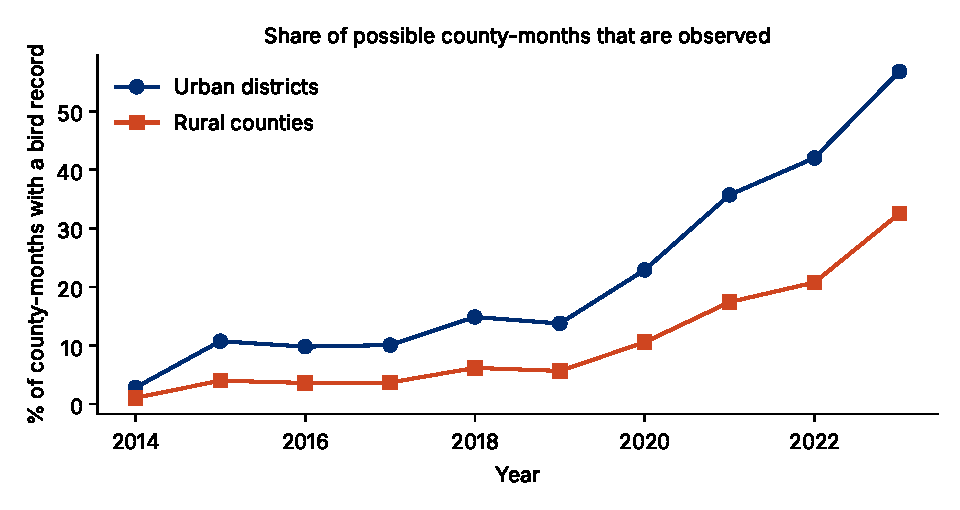
\includegraphics[width=0.78\linewidth]{../figures/5_4_observed_share_by_year.pdf}
\end{center}
\vspace{-6pt}
{\small\textit{Reading the figure:} the share of possible county-months with a bird record rose from about 2\% in 2014 to 41\% in 2023. Urban districts are always observed about twice as often as rural counties (57\% vs 33\% in 2023).}

\begin{center}
\footnotesize
\setlength{\tabcolsep}{3pt}
\begin{tabular}{l l c c c}
\toprule
Outcome & Version & Effect of +1 PSI & $p$ & Mean of outcome \\
\midrule
Observed (0/1), county-month & Paper FE & $-0.0055$ (0.0009) & $<0.001$ & 0.144 \\
 & Only counties ever observed & $-0.0070$ (0.0009) & $<0.001$ & 0.157 \\
 & Urban $\times$ YM FE & $+0.0001$ (0.0008) & 0.92 & 0.144 \\
 & Real-PSI counties only & $+0.0002$ (0.0008) & 0.79 & 0.113 \\
\addlinespace
ln(1 + birdwatchers), county-month & Paper FE & $-0.0167$ (0.0021) & $<0.001$ & 0.205 \\
 & Urban $\times$ YM FE & $-0.0016$ (0.0018) & 0.36 & 0.205 \\
 & Real-PSI counties only & $-0.0008$ (0.0017) & 0.67 & 0.146 \\
\addlinespace
Months observed (0--12), county-year & Paper FE & $-0.066$ (0.010) & $<0.001$ & 1.73 \\
 & Urban $\times$ year FE & $+0.001$ (0.010) & 0.92 & 1.73 \\
 & Real-PSI counties only & $+0.003$ (0.010) & 0.79 & 1.36 \\
\addlinespace
Any month observed, county-year & Paper FE & $+0.0029$ (0.0015) & 0.06 & 0.44 \\
 & Urban $\times$ year FE & $+0.0027$ (0.0016) & 0.08 & 0.44 \\
\addlinespace
Months observed, if $\ge 1$ & Paper FE & $-0.105$ (0.016) & $<0.001$ & 3.95 \\
 & Urban $\times$ year FE & $-0.032$ (0.016) & 0.049 & 3.95 \\
 & Real-PSI counties only & $-0.028$ (0.017) & 0.10 & 3.39 \\
\bottomrule
\multicolumn{5}{l}{\footnotesize County-month: 325,920 rows (233,640 real-PSI). County-year: 27,160 rows. SEs clustered by county.}
\end{tabular}
\end{center}

\textbf{What it means.}
\begin{itemize}[leftmargin=14pt,itemsep=1pt]
\item \textbf{Size.} In the paper's comparison, one standard deviation of PSI (3.4 points) lowers the chance a month is observed by about 1.9 percentage points, against a mean of 14.4\%. That is a 13\% relative drop, so missingness is clearly \emph{not} independent of PSI in the paper's design.
\item \textbf{Same pattern as the main result.} With urban $\times$ year-month FE, or in counties with real PSI data, the effect is essentially zero. Urban districts, most of which have PSI $=0$ imputed, saw much faster growth in birding than rural counties. In the paper's comparison PSI picks up ``rural'', and rural places are observed less.
\item \textbf{Intensive margin.} Among county-years with some observation, higher PSI still goes with slightly fewer observed months, even within the fair comparisons ($-0.03$ months, $p=0.05$ and $p=0.10$). This is weak evidence that policy years are observed a little less thoroughly.
\item \textbf{Bottom line.} Selection into the sample follows the same urban--rural split that produces the main estimate. Any analysis of these data should either compare like with like (urban $\times$ time FE) or model the chance of being observed. One option is to weight observed months by the inverse of their predicted probability of being observed.
\end{itemize}

%==========================================================================
\section{Item 3: solar-plant area as the treatment}
%==========================================================================
\textbf{Question.} What if the treatment is the \emph{physical} solar development, the land area of centralized PV plants, instead of the policy index?

\textbf{Why it matters.} Birds respond to land cover, not to documents. If PSI matters for birds, it should be \emph{because} it leads to solar plants. The authors run this once (Table S12, column 1: $-0.0387$). We apply the same checks we applied to PSI.

\textbf{Data facts first.}
\begin{itemize}[leftmargin=14pt,itemsep=1pt]
\item Area comes from the capacity file \texttt{IC.dta} (1,430 counties, 2009--2024). It is cumulative, so it is a \emph{stock}: it can only grow.
\item Only 1,317 of the 2,501 sample counties are in that file. For the other 1,184 counties (25,386 rows, 54.6\%) the authors set Area $=0$. This is the same imputation problem as with PSI.
\item 36.6\% of rows have Area $>0$: 46.8\% of rural rows but only 27.3\% of urban rows. So Area is again correlated with being rural.
\item One standard deviation of Area is 1.1 km$^2$.
\end{itemize}

\textbf{How.} \texttt{5\_5\_pv\_area\_treatment.do} runs five groups of checks:
\begin{enumerate}[label=\Alph*,leftmargin=18pt,itemsep=1pt]
\item different comparison groups;
\item different functional forms;
\item timing (lags and a lead);
\item effort and measurement;
\item the link between PSI and Area within a county.
\end{enumerate}

\begin{center}
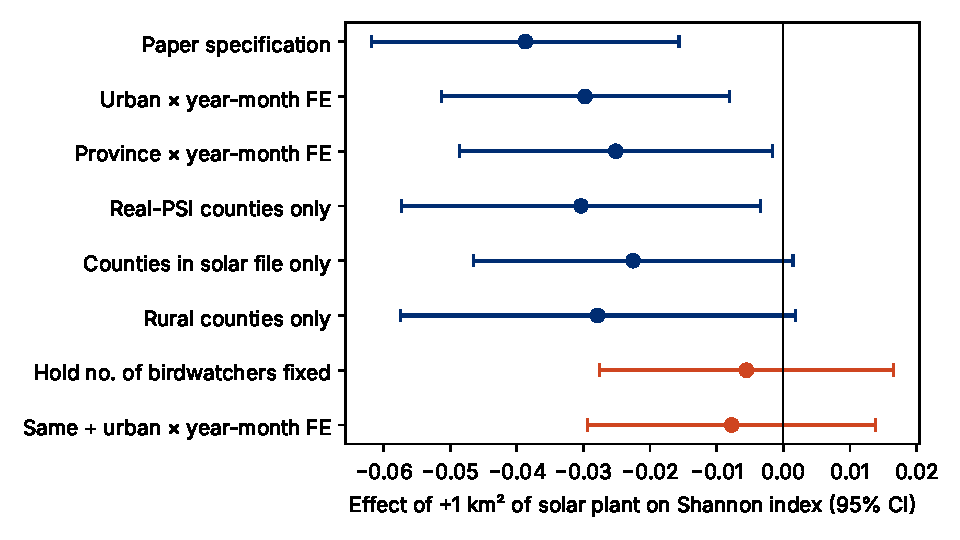
\includegraphics[width=0.82\linewidth]{../figures/5_5_area_coefplot.pdf}
\end{center}

\begin{center}
\small
\begin{tabular}{l c c r}
\toprule
Specification (outcome ShannonBD unless stated) & Effect of +1 km$^2$ & $p$ & Rows \\
\midrule
\multicolumn{4}{l}{\textit{A. Comparison groups}}\\
Paper (Table S12, col.\ 1) & $-0.0387$ (0.0118) & 0.001 & 46,371 \\
Urban $\times$ year-month FE & $-0.0298$ (0.0110) & 0.007 & 46,371 \\
Province $\times$ year-month FE & $-0.0251$ (0.0120) & 0.036 & 46,076 \\
Counties in the solar file only & $-0.0225$ (0.0122) & 0.066 & 21,054 \\
\quad same, urban $\times$ year-month FE & $-0.0207$ (0.0116) & 0.075 & 21,054 \\
Real-PSI counties only & $-0.0304$ (0.0137) & 0.027 & 26,007 \\
Rural counties only & $-0.0279$ (0.0151) & 0.066 & 22,164 \\
\multicolumn{4}{l}{\textit{B. Functional form}}\\
ln(1 + Area) & $-0.161$ (0.034) & $<0.001$ & 46,371 \\
Any centralized plant (0/1) & $-0.061$ (0.033) & 0.068 & 46,371 \\
\quad same, urban $\times$ year-month FE & $-0.047$ (0.034) & 0.166 & 46,371 \\
\multicolumn{4}{l}{\textit{C. Timing}}\\
Area one year earlier & $-0.0725$ (0.0215) & 0.001 & 46,371 \\
Area two years earlier & $-0.0733$ (0.0237) & 0.002 & 46,371 \\
Area one year \emph{later} (placebo) & $-0.0217$ (0.0088) & 0.014 & 46,371 \\
\quad placebo, with current Area also included & $-0.0039$ (0.0103) & 0.71 & 46,371 \\
Area, with PSI also included & $-0.0387$ (0.0118) & 0.001 & 46,371 \\
\multicolumn{4}{l}{\textit{D. Effort and measurement}}\\
Outcome: ln(birdwatchers) & $-0.0843$ (0.0223) & $<0.001$ & 46,371 \\
Outcome: ln(birdwatchers), urban $\times$ YM FE & $-0.0549$ (0.0181) & 0.003 & 46,371 \\
Shannon, holding ln(birdwatchers) fixed & $-0.0055$ (0.0113) & 0.62 & 46,371 \\
\quad same, urban $\times$ YM FE & $-0.0077$ (0.0110) & 0.48 & 46,371 \\
Outcome: richness (number of species) & $-1.83$ (0.62) & 0.003 & 45,606 \\
Outcome: evenness & $+0.0039$ (0.0026) & 0.13 & 43,958 \\
Shannon from months with $\ge$5 birding hours & $-0.0262$ (0.0157) & 0.097 & 22,314 \\
Outcome: month observed (full grid), paper FE & $-0.0099$ (0.0038) & 0.008 & 325,920 \\
\quad same, urban $\times$ YM FE & $-0.0027$ (0.0036) & 0.45 & 325,920 \\
\bottomrule
\multicolumn{4}{l}{\footnotesize SEs clustered by county. All models include the paper's controls, county FE and year-month FE.}
\end{tabular}
\end{center}

\textbf{E. Is PSI related to Area within a county?} Using real-PSI county-years (2014--2023), with county and year FE, +1 PSI point goes with $-0.035$ km$^2$ of solar area the same year, $-0.062$ one year later and $-0.054$ two years later (all $p<0.01$). Within a county, years with more policy are \emph{not} years of more solar construction. The paper supports PSI as a proxy for solar development with a pooled correlation ($r=0.041$) and a binned scatter plot (Fig.~S2). Both mix differences \emph{between} counties and include the imputed zeros. Within a county over time, which is the variation TWFE uses, the link is negative.

\textbf{What it means.}
\begin{itemize}[leftmargin=14pt,itemsep=1pt]
\item \textbf{Area survives the comparison-group checks better than PSI.} With urban $\times$ year-month or province $\times$ year-month FE, and in real-PSI counties, the Area estimate stays negative and significant at 5\%. This is the strongest evidence so far in favour of the paper's story.
\item \textbf{But it fails the effort check.} One more km$^2$ of solar plant goes with 8.4\% fewer birdwatchers (5.5\% within urban/rural groups). Holding birdwatchers fixed, the Area effect falls by about 85\% and is far from significant.
\item \textbf{Richness falls, evenness does not.} About 1.8 fewer species are recorded per km$^2$, while evenness does not change. Fewer observers mainly produce shorter species lists, so this is what a measurement effect would look like. A real habitat effect could also do it, so it is suggestive, not proof.
\item \textbf{Timing.} The ``one year later'' placebo is significant on its own. But Area is a growing stock, so next year's Area is almost the same as this year's. With current Area included, the placebo goes to zero. The test is uninformative rather than reassuring. A proper event study on the first year a county gets a plant (Task~3 methods) would be the clean test.
\item \textbf{Imputation.} In the 1,317 counties that really appear in the solar file, the estimate is smaller ($-0.022$) and only significant at 10\%.
\item \textbf{Bottom line.} Solar-plant area is the better treatment conceptually, and its link with lower recorded diversity is more robust than PSI's. But it moves together with birdwatching effort, so the same question remains: fewer birds, or fewer people looking? Data from fixed survey sites (item 7) would answer it.
\end{itemize}

%==========================================================================
\section{Item 4: weak instruments and Anderson--Rubin inference}
%==========================================================================
\subsection{The IV design in one paragraph}
The paper instruments PSI with
\[
Z_{it} = \frac{\ln(\text{mean sunshine hours } 1984\text{--}2013)_i}{\text{city climate-policy uncertainty}_{c(i)t}} .
\]
The idea: sunnier counties are better places for solar, so their policy reacts more strongly when national climate policy becomes \emph{less} uncertain. Two conditions are needed:
\begin{itemize}[leftmargin=14pt,itemsep=1pt]
\item \textbf{relevance:} $Z$ really moves PSI;
\item \textbf{exclusion:} $Z$ affects bird records \emph{only} through PSI.
\end{itemize}
The paper's 2SLS estimate is $-0.126$, ten times the TWFE estimate ($-0.0125$).

\subsection{How strong is the instrument?}
\texttt{5\_6\_weak\_iv\_anderson\_rubin.do}, part 1. With one instrument, the Kleibergen--Paap F that \texttt{ivreghdfe} reports \emph{is} the Montiel Olea--Pflueger effective F. Part 3 confirms this with \texttt{weakivtest}.

\begin{center}
\small
\begin{tabular}{l c c c c c}
\toprule
Version & 2SLS & SE & Clusters & Effective F & Passes 23.1? \\
\midrule
Paper: cluster county & $-0.126$ & 0.035 & 2,077 & 30.2 & \textcolor{good}{yes} \\
Cluster city (level of the CPU shock) & $-0.107$ & 0.047 & 287 & 10.8 & \textcolor{jhuorange}{no} \\
Cluster province & $-0.126$ & 0.093 & 27 & 2.8 & \textcolor{jhuorange}{no} \\
Urban $\times$ YM FE, cluster county & $-0.148$ & 0.047 & 2,077 & 22.3 & \textcolor{jhuorange}{borderline no} \\
Urban $\times$ YM FE, cluster city & $-0.122$ & 0.067 & 287 & 6.5 & \textcolor{jhuorange}{no} \\
Real-PSI counties, cluster county & $-0.117$ & 0.040 & 1,411 & 20.9 & \textcolor{jhuorange}{no} \\
Real-PSI counties, cluster city & $-0.089$ & 0.050 & 275 & 6.4 & \textcolor{jhuorange}{no} \\
\bottomrule
\multicolumn{6}{l}{\footnotesize City-clustered rows: 37,372 (131 rows have no city name). Other rows: 37,503; real-PSI: 19,985.}
\end{tabular}
\end{center}

\textbf{Which clustering is right?} The time-varying part of the instrument, city CPU, is the same for every county in a city in a given year. Rows in the same city share the same shock, so their errors are related. Clustering by city is the natural choice; this is the standard advice for shift-share instruments (Ad\~ao, Koles\'ar and Morales, 2019). By that standard the instrument is weak (F $\approx$ 11). None of the versions comes close to the 104.7 needed for the usual $\pm1.96$ interval (Lee et al., 2022).

\begin{answerbox}
\textbf{Where does ``F $\approx$ 8'' come from?} Table S10 of the supplement has a row ``F-statistic'' with values 8.78 and 8.00 under the first stages. That is the \emph{joint} F of all ten regressors (the instrument plus nine controls) printed by \texttt{reghdfe}, not the instrument's strength. Re-running column 4 gives a joint F of 8.00, while the instrument's own F is $(0.2054/0.0293)^2 = 49.0$. For column 2 it is $(0.0291/0.0044)^2 \approx 44$. For the main first stage (Table S7) the joint F is 6.3 and the instrument F 30.2. So the supplement's ``8'' does not mean the instrument is weak. The city-clustered F of 10.8 is the number that raises that concern.
\end{answerbox}

\subsection{Anderson--Rubin confidence sets}
\textbf{The idea, step by step.}
\begin{enumerate}[leftmargin=18pt,itemsep=1pt]
\item Pick a candidate effect $\beta_0$ (say $-0.05$).
\item Build $\tilde Y = \text{Shannon} - \beta_0 \times \text{PSI}$. If $\beta_0$ is the true effect, $\tilde Y$ no longer contains any PSI effect, so the instrument should not predict it.
\item Regress $\tilde Y$ on $Z$ with the same controls and FE, and test whether $Z$'s coefficient is 0 (clustered F-test). This is the AR statistic.
\item If the test does not reject at 5\%, keep $\beta_0$.
\item Repeat for a fine grid of $\beta_0$ values (step 0.001). The kept values form the AR 95\% confidence set.
\end{enumerate}
The first-stage strength never enters the test, so it is valid however weak the instrument is. With one instrument it is also the most powerful test of its kind, which is why Keane and Neal (2024) recommend it. Testing $\beta_0 = 0$ is the same as testing the reduced form.

\begin{center}
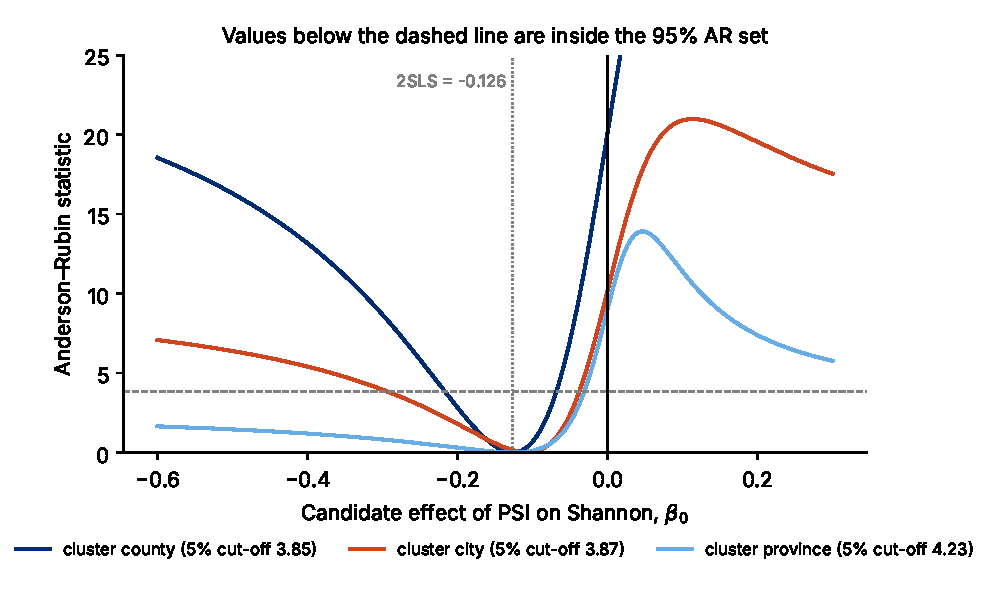
\includegraphics[width=0.82\linewidth]{../figures/5_6_anderson_rubin_curve.pdf}
\end{center}
\vspace{-4pt}
{\small\textit{Reading the figure:} each curve is the AR statistic for one way of clustering. Candidate effects where a curve is below the dashed line ($\approx$3.9) are kept. The province curve never rises above the line on the left, so its set extends to $-\infty$.}

\begin{center}
\small
\begin{tabular}{l c c c}
\toprule
Version & Usual 95\% CI & AR 95\% set & AR $p$ for $\beta=0$ \\
\midrule
Paper: cluster county & $[-0.194, -0.059]$ & $[-0.217, -0.068]$ & $<0.001$ \\
Cluster city & $[-0.199, -0.015]$ & $[-0.295, -0.037]$ & 0.002 \\
Cluster province & $[-0.317, +0.064]$ & $(-\infty, -0.028] \cup [0.586, +\infty)$ & 0.006 \\
Urban $\times$ YM FE, cluster county & $[-0.240, -0.056]$ & $[-0.282, -0.072]$ & $<0.001$ \\
Urban $\times$ YM FE, cluster city & $[-0.253, +0.009]$ & $[-0.601, -0.033]$ & 0.004 \\
Real-PSI, cluster county & $[-0.195, -0.039]$ & $[-0.234, -0.053]$ & $<0.001$ \\
Real-PSI, cluster city & $[-0.187, +0.010]$ & $[-0.466, -0.024]$ & 0.003 \\
\bottomrule
\end{tabular}
\end{center}

\textbf{What it means.}
\begin{itemize}[leftmargin=14pt,itemsep=1pt]
\item Every AR set excludes zero. When the instrument is weak (city or province clustering), the sets become wide, and with 27 province clusters the set is unbounded, but they never include zero. Several versions whose usual CI includes zero (province, and city with urban $\times$ YM FE or real-PSI) still reject zero under AR.
\item So \textbf{a weak instrument is not the reason to doubt the IV}. The reduced form is clearly negative: sunnier counties record lower Shannon when city CPU falls.
\item \textbf{But AR assumes exclusion holds.} If $Z$ affects bird records directly, every number above is wrong, AR included.
\end{itemize}

\subsection{The exclusion restriction: plausibly exogenous IV}
In Task 1 (\texttt{1\_6}, Panel A) we ran the zero-first-stage test. In the 724 counties whose PSI is imputed as 0, $Z$ \emph{cannot} move PSI, yet $Z$ still predicts lower Shannon: $\hat\gamma = -0.00214$ (SE 0.00108, $p=0.048$). That is a direct effect of the instrument, which exclusion rules out.

Part 6 of the do-file subtracts this direct effect, $\tilde Y = \text{Shannon} - \gamma Z$, and re-runs 2SLS (Conley et al., 2012; van Kippersluis and Rietveld, 2018):

\begin{center}
\small
\begin{tabular}{l c c c}
\toprule
Assumed direct effect $\gamma$ & IV estimate & SE & AR 95\% set \\
\midrule
$\gamma=0$ (paper's assumption) & $-0.126$ & 0.035 & $[-0.217, -0.068]$ \\
$\gamma=-0.00214$ (estimate) & $-0.042$ & 0.029 & $[-0.105, +0.014]$ \\
$\gamma=-0.00425$ (lower end of its 95\% CI) & $+0.042$ & 0.030 & $[-0.013, +0.114]$ \\
$\gamma=-0.00002$ (upper end) & $-0.125$ & 0.035 & $[-0.216, -0.067]$ \\
\bottomrule
\end{tabular}
\end{center}

\textbf{What it means.} The reduced form is $-0.00319$. About two-thirds of it ($-0.00214$) also appears where PSI cannot respond. Taking that direct effect out cuts the IV estimate by two-thirds, and the estimate is no longer distinguishable from zero.

Caution: $\gamma$ is measured in counties that are mostly urban, and the direct effect may be different elsewhere. Even so, this is concrete evidence that the IV's problem is \textbf{exclusion}, not strength. A likely channel is that climate-policy uncertainty in a city affects other things that change bird records, such as other environmental policy, land use and birding activity. In Task 1 the instrument predicted several of these.

\begin{answerbox}
\textbf{Answer to item 4.}
\begin{itemize}[leftmargin=14pt,itemsep=1pt,topsep=2pt]
\item The instrument is strong only with county clustering (effective F 30.2). It is weak with city clustering, which is the natural level for this shift-share design (10.8), and very weak with province clustering (2.8).
\item Anderson--Rubin sets, which are valid with weak instruments, still exclude zero in every version.
\item Allowing for the direct effect we measured where the first stage is zero reduces the IV estimate to about $-0.04$ and makes it insignificant. The IV evidence therefore depends on the exclusion restriction, and our data cast doubt on it.
\end{itemize}
\end{answerbox}

%==========================================================================
\section{Item 7: fixed-site bird monitoring data}
%==========================================================================
\textbf{Why it matters.} Every problem above comes from the bird data being opportunistic citizen science: where and when people go birding is not controlled. Standardized surveys repeat the same routes, at the same season, with the same method. That fixes effort, so a change in counts reflects a change in birds.

\textbf{What exists.}
\begin{center}
\small
\begin{tabularx}{\linewidth}{>{\raggedright\arraybackslash}p{3.1cm} >{\raggedright\arraybackslash}X >{\raggedright\arraybackslash}p{3.3cm}}
\toprule
\textbf{Source} & \textbf{Design and coverage} & \textbf{Access / fit} \\
\midrule
China BON-Birds (national) & Run by the Nanjing Institute of Environmental Sciences, Ministry of Ecology and Environment, since 2011. Fixed line transects of 1--3 km, surveyed in the breeding season (March--July), plus point counts at major wetlands in winter. Sites chosen by stratified random sampling across ecosystem types and elevations. Records species, number of individuals, coordinates, date, habitat and disturbance. The whole China BON network (birds, amphibians, mammals, butterflies) reports 441 sample regions and about 9,000 transects and points. & National raw data: by request to the institute. Best fit. \\
\addlinespace
China BON-Birds, Yangtze River Basin subset & 536 monitoring sites, 2011--2020, same protocol. Published with a study of bird-diversity trends in the basin. & \textbf{Public on Dryad} (doi:10.5061/\allowbreak dryad.\allowbreak np5hqbzzh). Overlaps our PSI years 2014--2020. \\
\addlinespace
China Coastal Waterbird Census & Volunteer-run since 2005. 32 coastal sites, 14 of them counted every month at high tide. & Coastal waterbirds only; reports via the Hong Kong Bird Watching Society. Not suitable for a national test. \\
\addlinespace
Local park monitoring (e.g.\ Shennongjia) & Fixed transects and points inside single protected areas. & Too few places. \\
\bottomrule
\end{tabularx}
\end{center}

\textbf{How it would be used.}
\begin{enumerate}[leftmargin=18pt,itemsep=1pt]
\item Download the Dryad subset; map each site to its county using the coordinates.
\item Compute site-year Shannon, richness and evenness. Effort is the same every year by design (same transect, same season, same method).
\item Regress site-year diversity on county solar-plant area (and PSI) with site and year fixed effects, clustered by county. Also run urban $\times$ year and province $\times$ year versions.
\item Compare the result with the citizen-science estimate for the same counties and years. If the effect survives at fixed sites, the effort explanation is ruled out. If it disappears, the paper's effect is likely an observation effect.
\end{enumerate}

\textbf{Limits.} The Yangtze subset covers one large basin (about a fifth of China) and 2014--2020 only. Site counts per county are small, so the test has less power than the paper's. The national network would need a formal data request.

%==========================================================================
\section{What the follow-ups add, and next steps}
%==========================================================================
\begin{enumerate}[leftmargin=18pt,itemsep=3pt]
\item \textbf{One confounder keeps appearing.} PSI is high in rural counties and imputed 0 in most urban districts. Urban birding grew much faster. This single fact explains the PSI effect on Shannon (Task 1), on effort (item 1) and on which months are observed (item 2). Within urban and within rural groups, PSI has no detectable effect on any of them.
\item \textbf{Solar-plant area is the most promising treatment.} Its negative association survives the comparison-group checks.
\item \textbf{Effort is the unresolved issue.} Both PSI and Area go with fewer birdwatchers, and holding birdwatchers fixed removes both effects. The data cannot separate ``fewer birds'' from ``fewer observers''.
\item \textbf{IV.} Strength is adequate only under county clustering, but AR inference keeps the reduced form significant. The real weakness is exclusion: correcting for the measured direct effect removes most of the IV estimate.
\end{enumerate}

\textbf{Possible next steps} (for discussion on Thursday):
\begin{itemize}[leftmargin=14pt,itemsep=1pt]
\item Event study on the first year a county gets a centralized solar plant (Callaway--Sant'Anna / BJS, as in Task 3). This replaces the uninformative lead test.
\item Inverse-probability weighting for observed months, using the full grid from \texttt{5\_4}.
\item Effort-standardized outcomes, e.g.\ species recorded per birdwatcher-hour, or rarefaction to a fixed number of records.
\item Download the China BON-Birds Yangtze subset (Dryad) and run the fixed-site test above; request the national data.
\item Anderson--Rubin and plausibly-exogenous bounds for the urban $\times$ YM and real-PSI IV versions, with city clustering.
\end{itemize}

%==========================================================================
\appendix
\section{References}
\begin{itemize}[leftmargin=14pt,itemsep=1pt]
\item Ad\~ao, R., Koles\'ar, M., Morales, E. (2019). Shift-share designs: theory and inference. \textit{Quarterly Journal of Economics} 134(4), 1949--2010.
\item Anderson, T.W., Rubin, H. (1949). Estimation of the parameters of a single equation in a complete system of stochastic equations. \textit{Annals of Mathematical Statistics} 20(1), 46--63.
\item Andrews, I., Stock, J.H., Sun, L. (2019). Weak instruments in instrumental variables regression: theory and practice. \textit{Annual Review of Economics} 11, 727--753.
\item Conley, T.G., Hansen, C.B., Rossi, P.E. (2012). Plausibly exogenous. \textit{Review of Economics and Statistics} 94(1), 260--272.
\item Keane, M., Neal, T. (2024). A practical guide to weak instruments. \textit{Annual Review of Economics} 16, 185--212.
\item Lee, D.S., McCrary, J., Moreira, M.J., Porter, J. (2022). Valid t-ratio inference for IV. \textit{American Economic Review} 112(10), 3260--3290.
\item Montiel Olea, J.L., Pflueger, C. (2013). A robust test for weak instruments. \textit{Journal of Business \& Economic Statistics} 31(3), 358--369.
\item van Kippersluis, H., Rietveld, C.A. (2018). Beyond plausibly exogenous. \textit{Econometrics Journal} 21(3), 316--331.
\item China BON (GEO BON network page): \url{https://geobon.org/china-bon-network/}.
\item China BON-Birds, Yangtze River Basin bird data, 2011--2020: Research Square preprint rs-2799008 (2023); data on Dryad, doi:10.5061/dryad.np5hqbzzh.
\item Progress in construction of China Bird Diversity Observation Network (China BON-Birds). \textit{Journal of Ecology and Rural Environment} (2018), doi:10.11934/j.issn.1673-4831.2018.01.001.
\item China Coastal Waterbird Census: \textit{Avian Research} (2015), doi:10.1186/s40657-015-0021-2.
\item Zhang et al.\ (2026). China's solar expansion policy reduces bird diversity. \textit{Science} 393, 831, and Supplementary Materials.
\end{itemize}

\section{Stata code}
Folder: \texttt{Solar\_Birds\_Replication/05\_Followups\_Nov13/}. Run \texttt{code/5\_0\_run\_followups.do}. It writes logs to \texttt{logs/}, tables to \texttt{tables/} and the county-month grid to \texttt{data/}. Every file starts from \texttt{00\_config.do} (paths, control lists, packages). Files \texttt{5\_1} and \texttt{5\_2} are the 13 November effort and dummy-variable checks.

\textbf{One-command demo.} \texttt{DEMO\_followups.do} runs all of the above live and stops after each step until you press Enter (type \texttt{q} to stop):
\begin{lstlisting}[numbers=none]
do "/Users/sahiljangra/Desktop/Johns Hopkins/RA/Solar_Birds_Replication/05_Followups_Nov13/DEMO_followups.do"
\end{lstlisting}
Running \texttt{ADD\_FOLLOWUP\_MENU.do} once adds a menu button, \textit{User $\rightarrow$ Solar Birds: Follow-ups (13 Nov)}, that starts the demo with one click.

\subsection{5\_0\_run\_followups.do}
\lstinputlisting{../code/5_0_run_followups.do}
\subsection{5\_1\_effort\_test.do}
\lstinputlisting{../code/5_1_effort_test.do}
\subsection{5\_3\_sample\_flow.do}
\lstinputlisting{../code/5_3_sample_flow.do}
\subsection{5\_4\_missingness\_test.do}
\lstinputlisting{../code/5_4_missingness_test.do}
\subsection{5\_5\_pv\_area\_treatment.do}
\lstinputlisting{../code/5_5_pv_area_treatment.do}
\subsection{5\_6\_weak\_iv\_anderson\_rubin.do}
\lstinputlisting{../code/5_6_weak_iv_anderson_rubin.do}
\subsection{DEMO\_followups.do}
\lstinputlisting{../DEMO_followups.do}
\subsection{code/demo\_programs.do (the demo steps)}
\lstinputlisting{../code/demo_programs.do}
\subsection{ADD\_FOLLOWUP\_MENU.do}
\lstinputlisting{../ADD_FOLLOWUP_MENU.do}
\subsection{5\_2\_sensitivity\_dummies.do}
\lstinputlisting{../code/5_2_sensitivity_dummies.do}

\end{document}
